\subsection{Verbesserungsideen}\label{subsec:verbesserungsideen}
Nachfolgend werden mögliche Verbesserungsideen in Bezug auf den Programmcode und dem DBMS aufgelistet und mittels konkreter Implementierung bzw. Umsetzung erläutert.
\subsubsection{Views}
Als erste Verbesserungsidee können Views in Betracht gezogen werden.
Diese sogenannten Database Views sind gespeicherte Abfragen, die beim Aufrufen eine Ergebnismenge erzeugen, wie eine virtuelle Tabelle.
Per Definition ist eine View eine benannte Abfrage, die im Datenbankkatalog gespeichert ist.

\subsubsection{Initialisierte Prepared-Statements}
Als zweite Verbesserung das Initialisieren der Prepared-Statements während dem Start.
Diese werden serverseitig vorbereitet, sodass nur noch die Platzhalter in der Abfrage mit den jeweiligen Parametern ersetzt werden müssen.
Dabei bieten Prepared-Statements folgende Vorteile: zum einen weniger Overhead für das Parsen der Anfragen bei jeder Ausführung und außerdem Schutz vor SQL-Injections, da die zuvor übermittelten Anweisungen nur an den Platzhaltern geändert werden können und nur mit den jeweiligen richtigen Parameter-Datentypen.
\subsubsection{Indices}
Indices in Relationen werden genutzt, um Tupel effizient mit bestimmten Werten zu finden.
Ohne einen Index für den zu suchenden Wert muss das MySQL-DBMS mit dem ersten Tupel beginnen und dann durch die gesamte Tabelle lesen.
Dementsprechend kann das DBMS durch die Indices in einer Tabelle schnell die Position finden, an der die Tupel voran weiter durchsucht werden sollen.

\subsubsection{Manuelles Commiten}
    Damit die Datenintegrität nur an semantisch sinnvollen Punkten sichergestellt wird, haben wir Autocommit deaktiviert.
    Dadurch wird nur an sinnvollen Stellen Aufwand wür die Überprüfung aufgebracht.

\subsubsection{Batches}
    Um mehrere Transaktionen in einem an das DBMS zu übermitteln wollten wir zunächst mit Batches optimieren.
    Diese Idee haben wir allerdings verworfen, da bei der verwendung von Prepared Statements, nicht mehrere verschiedene Prepared Statements demselben Batch hinzugefügt werden können.

\subsection{Programmcode}\label{subsec:programmcode}
\subsubsection{Views - Version 2}
Die Views wurden nur für die Kontostandtransaktion und der Analysetransaktion umgesetzt, da diese beiden ein SELECT-Statement ausführen, das sich für Database Views eignet.
Dabei muss vor der Nutzung der Views im Programmcode diese in der Datenbank hinterlegt werden, indem diese über die MySQL Workbench erstellt und an das DBMS gesendet werden.
\lstinputlisting[breaklines,language=SQL,label={lst:version2-createViewAccountsBalances},caption={SQL Statement zur Erstellung der View für die Kontostandtransaktion}]{assets/code/version2/createViewAccountsBalances.sql}
\lstinputlisting[breaklines,language=SQL,label={lst:version2-createViewAccountsBalanceNumbers},caption={SQL Statement zur Erstellung der View für die Analysetransaktion}]{assets/code/version2/createViewAccountsBalanceNumbers.sql}

\subsubsection{Initialisierte Prepared-Statements - Version 3}
Das Initialisieren der Prepared-Statements während dem Start verbessert die Performance der einzelnen Transaktionen (Kontostand-TX und Analyse-TX).
Siehe \hyperref[subsec:version3]{\textbf{Dokumentation-Version 3}}.

\subsubsection{Indices - Version 4}
Um einen weiteren Index in der Relation history mit dem Verweis auf accbalance zu erstellen muss die untere SQL-Anweisung ausgeführt werden.
\lstinputlisting[breaklines,language=SQL,label={lst:version4-createIndexAccbalanceInHistory},caption={SQL Statement zur Erstellung des Index für accbalance in der Relation history}]{assets/code/version4/createIndexAccbalanceInHistory.sql}
Hierbei wird ein Index für accbalance erstellt, der für die Analyse-TX genutzt wird, um die einzelnen Beträge (accbalance) in der View (accounts\_balance\_numbers) zu gruppieren, zu vergleichen und die Anzahl dieser zurückzuliefern.

\begin{figure}[h!]
    \center
    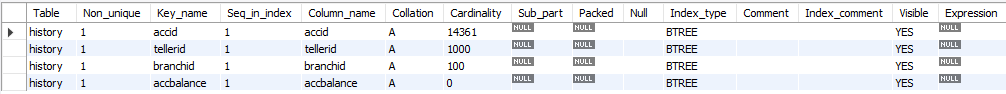
\includegraphics[width=\linewidth]{assets/img/database-history-indices}
    \caption{DBMS - Indices in history Relation}
    \label{fig:database-indices-history}
\end{figure}
\begin{center}

\end{center}
\subsection{Datenbankmanagementsystem}\label{subsec:datenbankmanagementsystem}